
\chapter{Measuring Luminosity}

\section{Instantaneous Luminosity}

One of the most important quantities measured by CMS is luminosity. Luminosity is necessary to convert the number of events detected, for a given channel, into a collision cross-section. Collision cross-sections are among the primary observables predicted by theoretical physics, specifically quantum field theory. For particle physics, the collision cross-section of a process is typically measured through the relation:
\begin{equation}
\sigma  = \frac{R}{\mathit{L}} ,
\end{equation}
where $\sigma$ is the cross-section, $R$ is the rate at which the process occurs per collision, and $L$ is the luminosity.

\section{Luminometers}

There are two kinds of CMS luminometer: online and offline. Online luminometers readout the luminosity per bunch in real time. As of 2015 there are three online luminometers: the pixel luminosity telescope (PLT), the HF, and the beam conditions monitor (BCM1f). There is a high-rate, independent data-acquisition system for each of the online luminometers. Offline luminometers measure the rate of reconstructed objects. The primary offline lumimoneter is the pixel tracker. In general, the offline lumimometers have better stability over time. \cite{CMS:2010gua}

The online and offline luminometers complement each other for high precision data analysis. Specifically, the offline data can be used to calibrate out imperfections in the online data. 

In addition to these hardware luminometers, CMS can use physics processes as luminosity benchmarks.  For example, other experiments have measured the Z-boson cross-section to a high accuracy and high precision. Comparing this cross-section to the Z-boson mass-peak ,in CMS data, provides a cross-check to the delivered luminosity. 

\section{Van de Meer Scanning Calibration}

The luminometers of CMS produce signals proportional to the instantanteous luminosity of the LHC beam. However, these signals need to be properly calibrated with respect to a known visible cross-section for each luminometer. This calibration is accomplished via Van de Meer scanning. The opposing beams of LHC are moved back and forth in the transverse plane. During the scan, the detector response is measured as a function of beam displacement. The beam widths are calculated from Gaussian fits to the detector response. The visible cross-section of the luminometer in question is then derived from the width of the beams, and acts as the calibration of the detector response. 

\begin{figure}[h!]
\begin{centering}
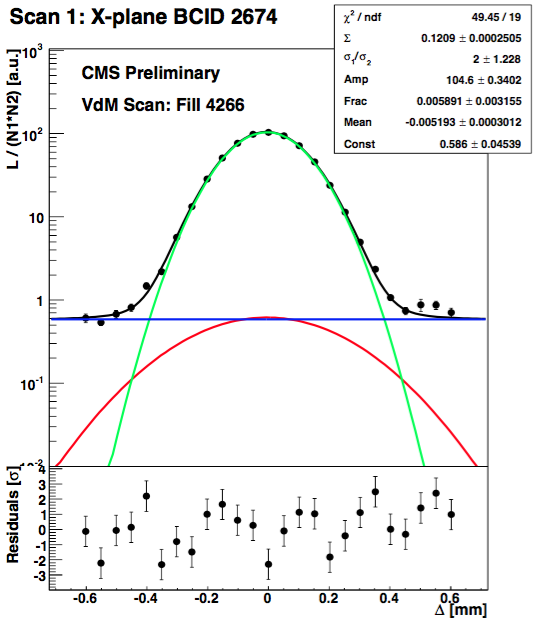
\includegraphics[width=3in]{Chapter4/importfigs/CMS-PAS-LUM-15-001_Figure_005-a.png}
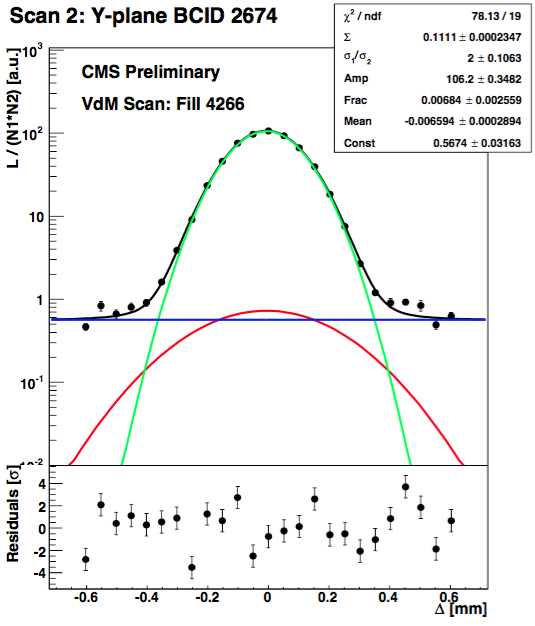
\includegraphics[width=3in]{Chapter4/importfigs/CMS-PAS-LUM-15-001_Figure_005-b.png}
\par\end{centering}
\caption{PCC VdM Scans. \label{fig:pccVdMScans}}
\end{figure}

\section{Comparitive Luminosity Performance of LHC Detectors}

\begin{figure}[h!]
\begin{centering}
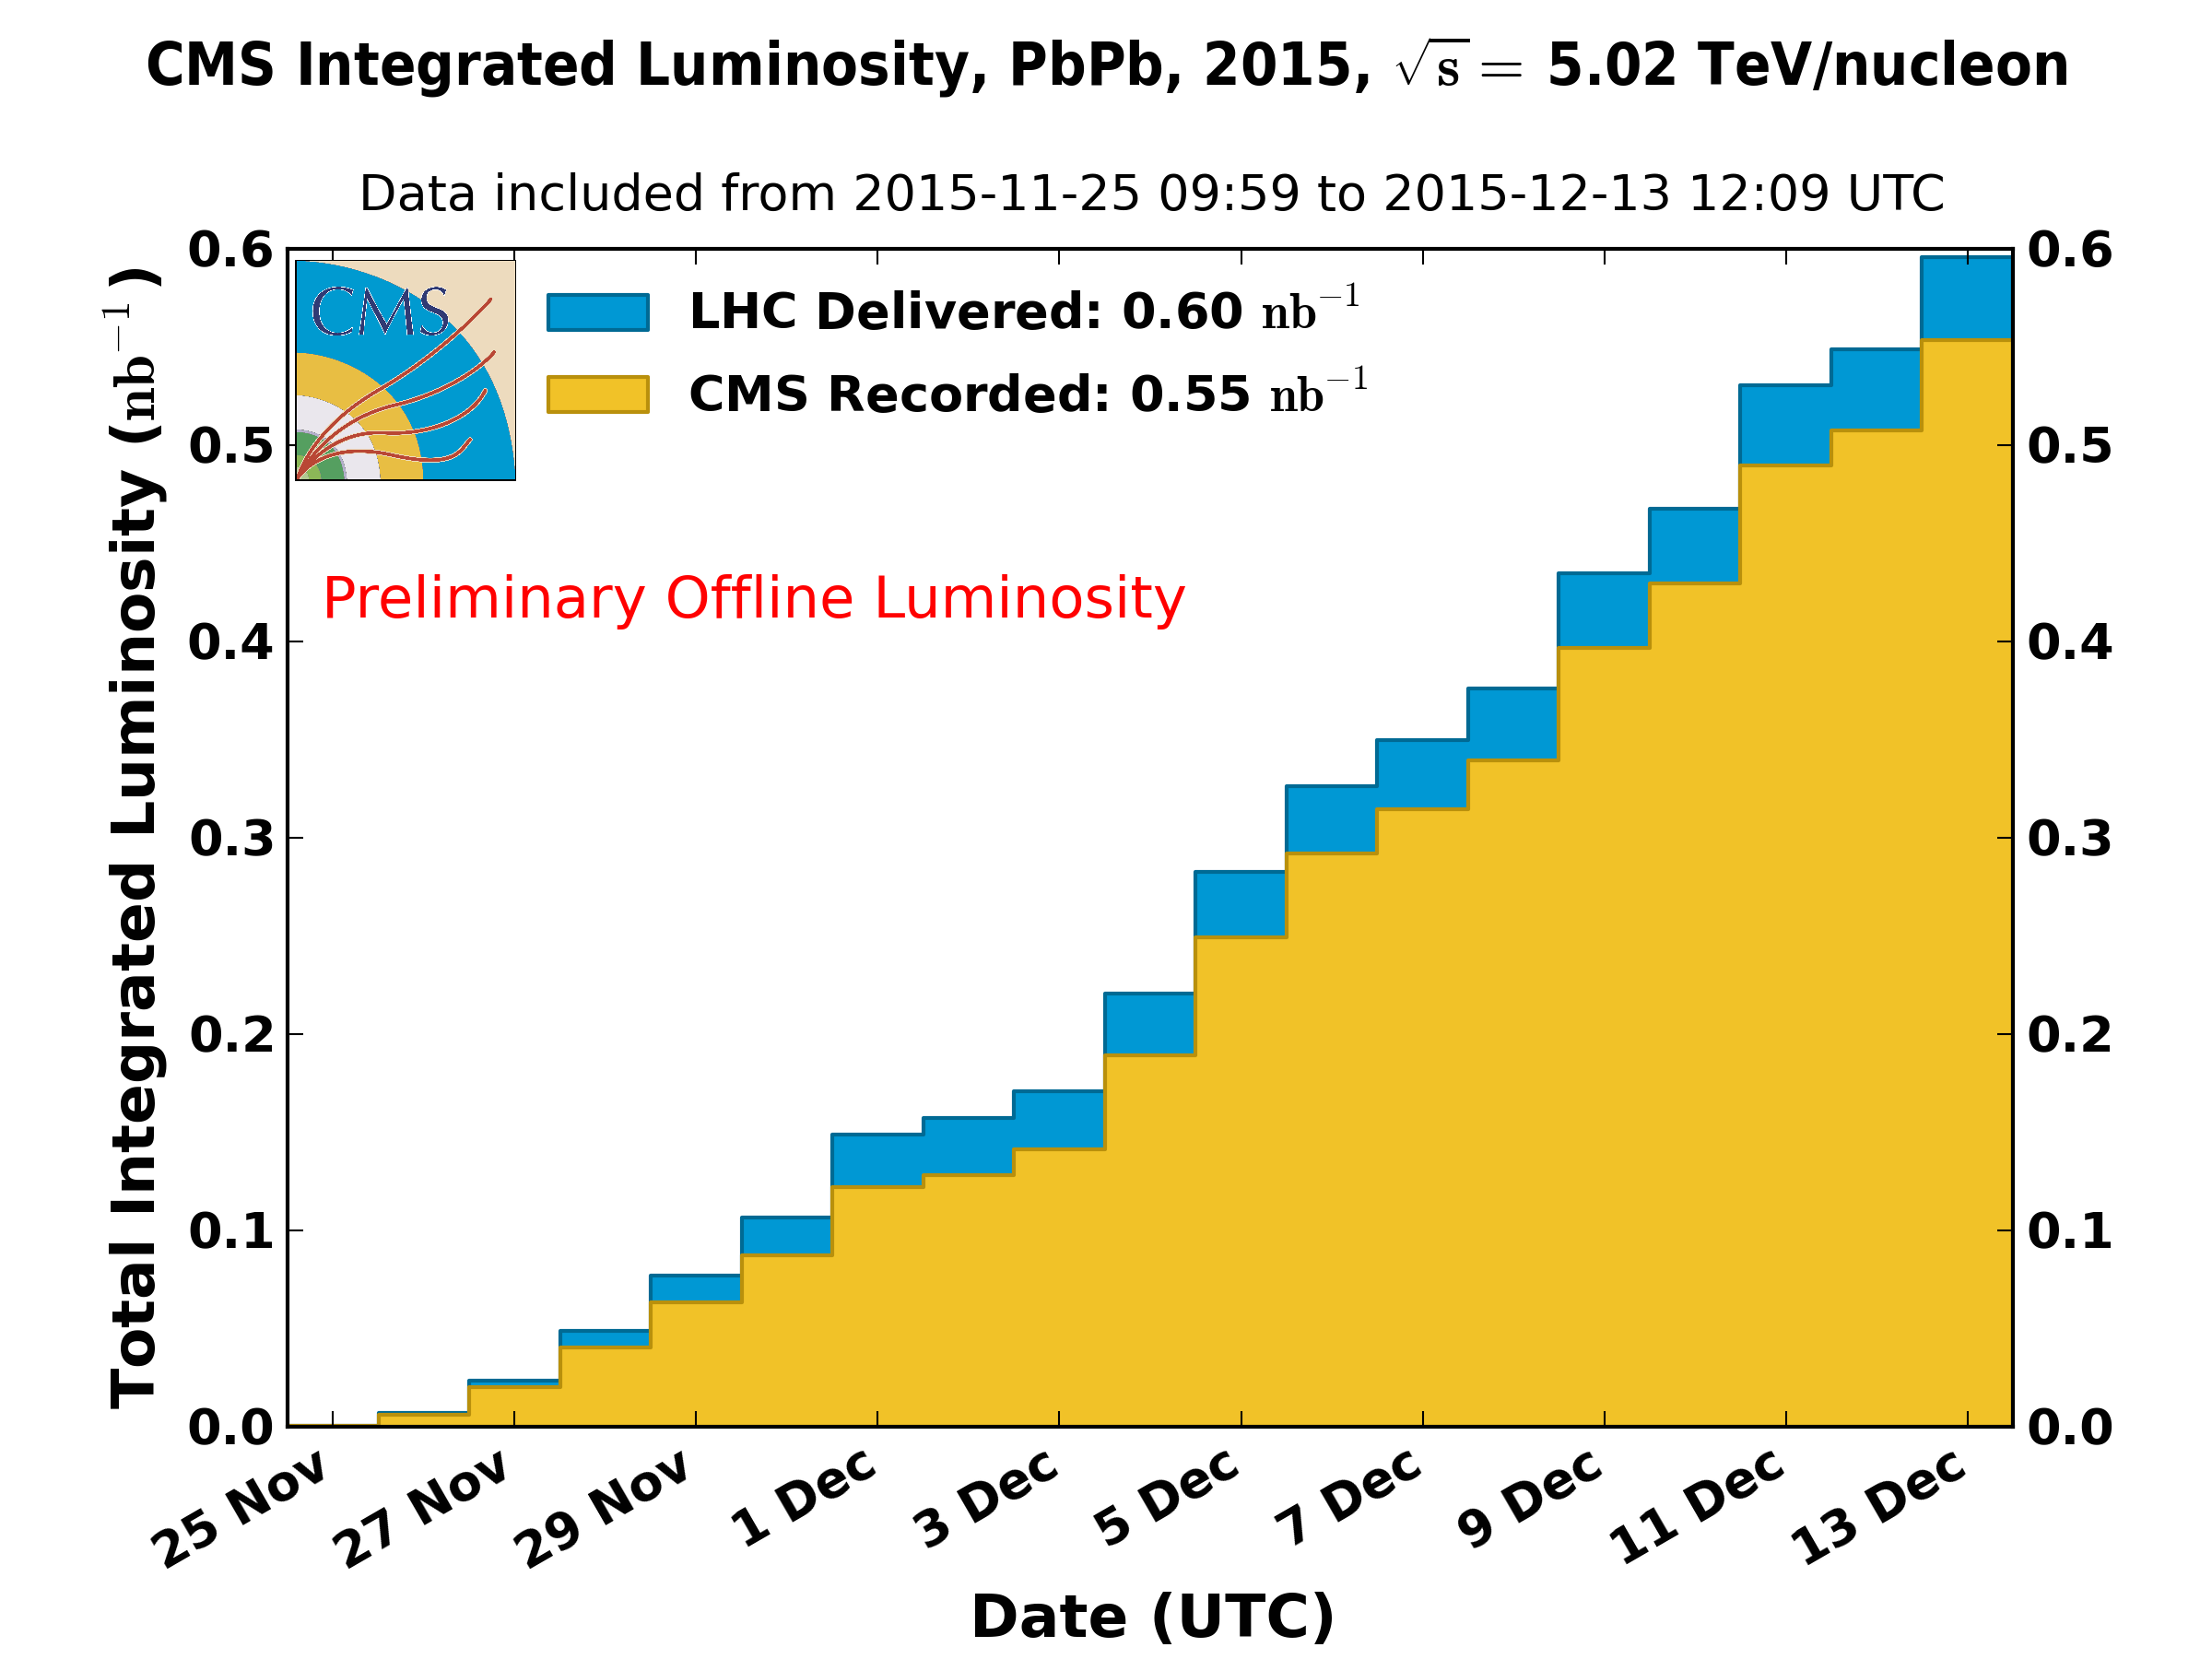
\includegraphics[width=6in]{Chapter4/importfigs/int_lumi_per_day_cumulative_pbpb_2015_pbpb.png}
\par\end{centering}
\caption{CMS lumi during HI-2015. \label{fig:lumiHi2015}}
\end{figure}

\begin{figure}[h!]
\begin{centering}
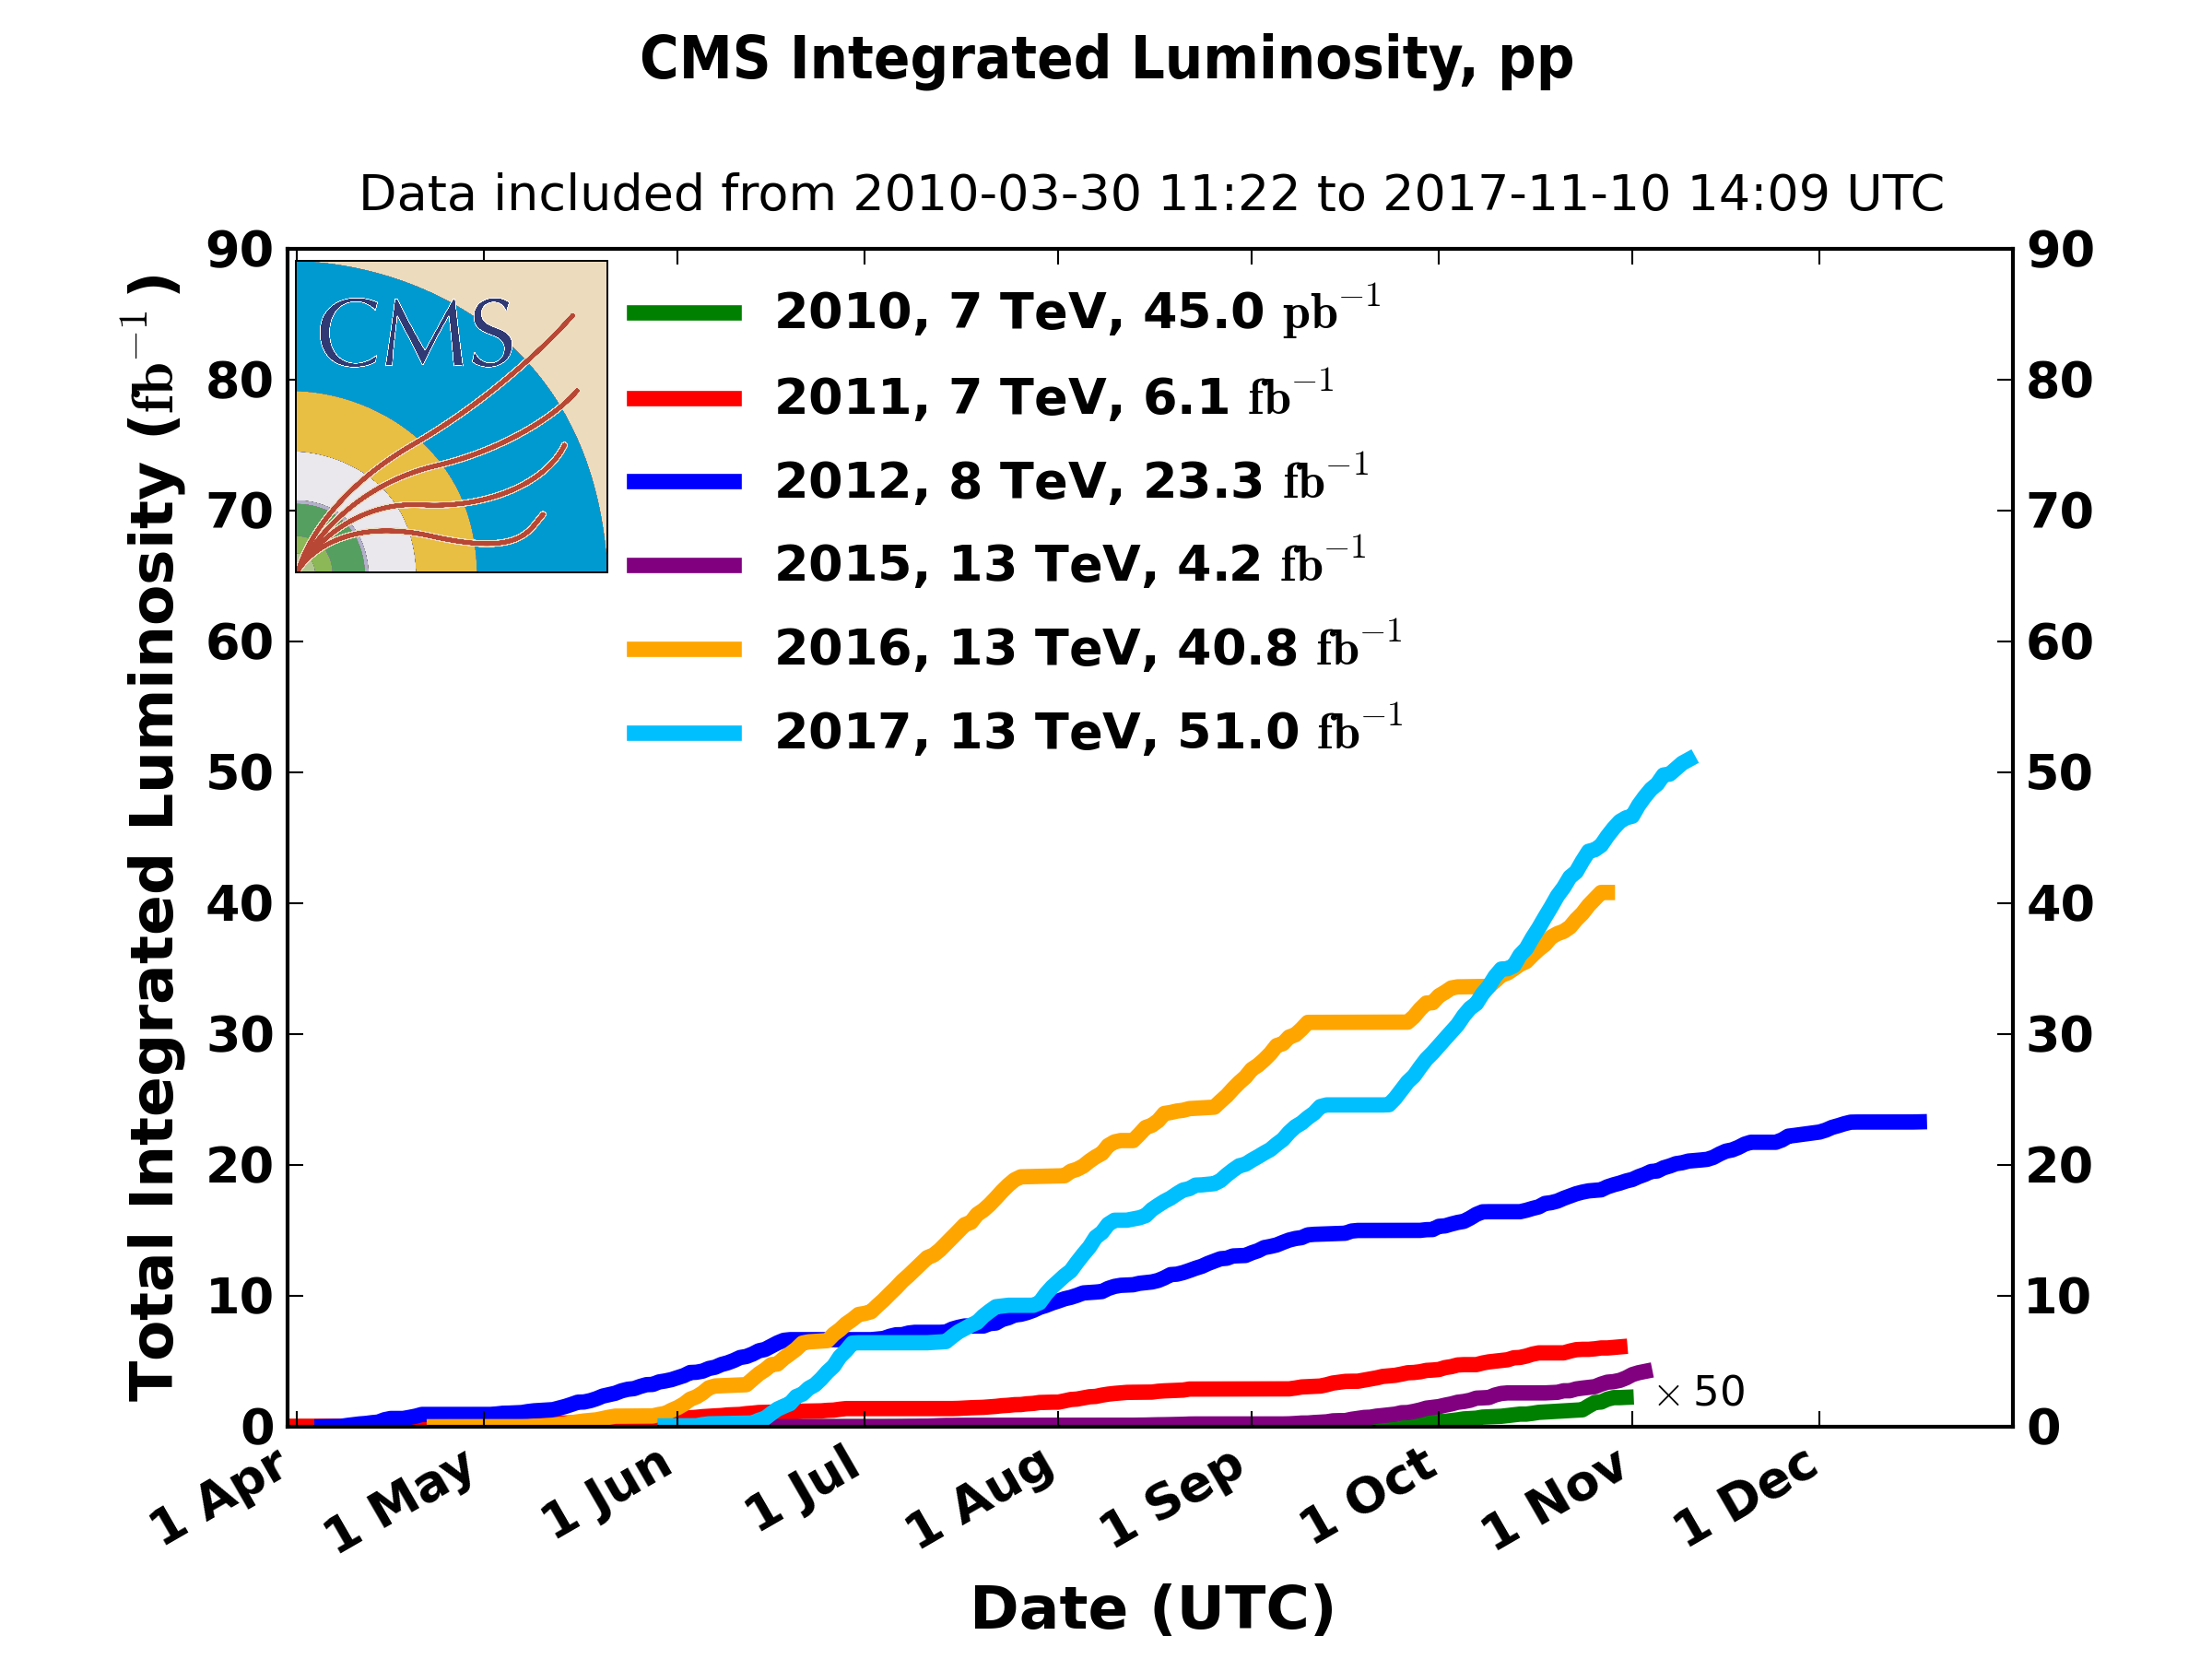
\includegraphics[width=6in]{Chapter4/importfigs/int_lumi_cumulative_pp_2.png}
\par\end{centering}
\caption{CMS Lumi by Era. \label{fig:lumiCMSEra}}
\end{figure}


\section{Systematic Uncertainty}

\begin{figure}[h!]
\begin{centering}
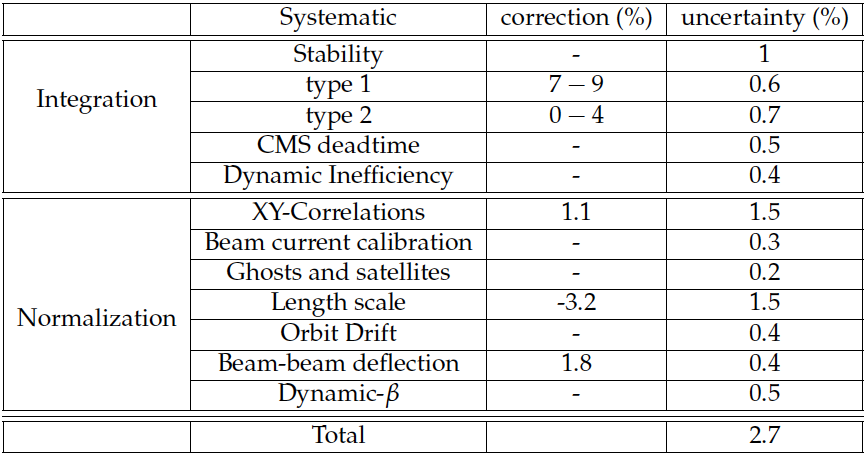
\includegraphics[width=4in]{Chapter4/importfigs/CMS-PAS-LUM-15-001_Table_001.png}
\par\end{centering}
\caption{Systematic Uncertainty During 2015 pp Run. \label{fig:sysLumiError}}
\end{figure}


\section{Author's Contributions}

LHC produces a staggering amount of data. The 2015 heavy-ion run itself recorded some $1.4 pb^-1$ in integrated luminosity. This integrated luminosity is reconstructed into data on the order of pentabytes. 

\begin{figure}[h!]
\begin{centering}
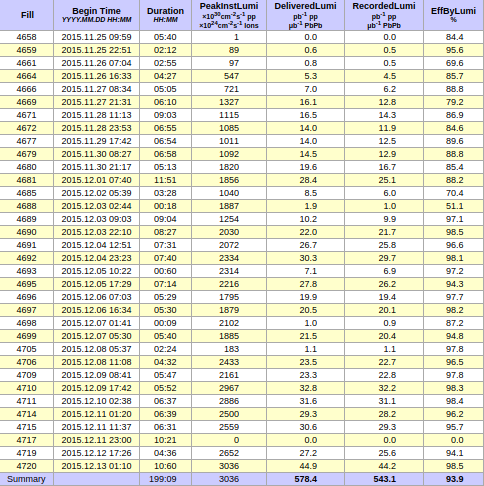
\includegraphics[width=6in]{Chapter4/importfigs/lumiFill.png}
\par\end{centering}
\caption{Luminosity by CMS fill. \label{fig:lumiFill}}
\end{figure}

I contributed to CMS luminosity validation, and performed studies on the long-term stability of the BRIL luminometers. On a week by week basis, I would examine the data from online and offline luminometers and certify that it met the quality standards of CMS. If the data exhitibed non-linear behavior, I would de-certify the corresponding lumi-sections in the BRIL json files.

All CMS data has to go through a data certification workflow. Data certification insures that only valid data is used in CMS analyses. Decisions on data certification are recorded in two systems: the DQM Run Registry, shown here in figure \ref{fig:runRegistry}, and the normtag JSON files of the BRIL-DPG. There are occasions when the sub-detectors of CMS might record poor quality data. For example, the software reading out data from the PLT could crash and thus compromise the output. In this case the certification workers would record the lumi sections during which the PLT software crashed. These lumi sections would be removed from the normtag JSON file passed on to the BRIL group. If all te luminometers are malfunctioning, a whole run could be invalidated in the run registry. 

\begin{figure}[h!]
\begin{centering}
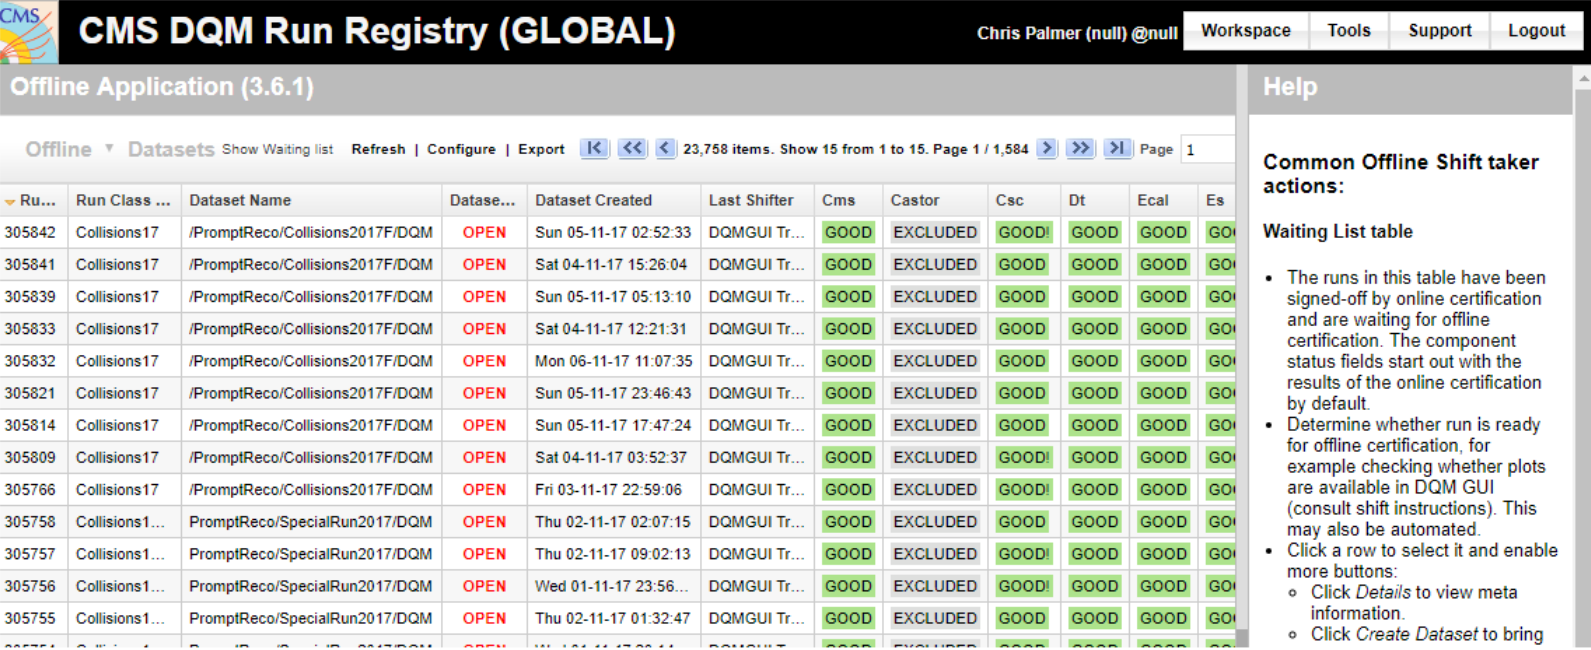
\includegraphics[width=6in]{Chapter4/importfigs/chris_palmer_run_registry.png}
\par\end{centering}
\caption{CMS Run Registry. \label{fig:runRegistry}}
\end{figure}

In additon to data certification, I reviewed the long-term stability of the BRIL luminometers during the 2015 and 2016 proton-proton runs. Stability refers to the comparative performance of the different luminometers. Ideally, the ratio of the instantaneous luminosity reported by separate luminometers should be a constant ratio, but in fact there is a tendency for this ratio to drift as a result of radiation damage to the luminometers. This drift can be seen in plotting the average ratio as a function of interaction rate and of the different measures of LHC time: runs, lumi-sections, and bunch-crossings.  Instantaneous luminosity, in theory, should be independent of machine conditions like acceptance and efficiency. 